\documentclass[conference]{IEEEtran}
\IEEEoverridecommandlockouts

\usepackage{amsmath,amssymb,amsfonts}
\usepackage{graphicx}
\usepackage{textcomp}
\usepackage{xcolor}
\usepackage[backend=biber,style=numeric]{biblatex}
\addbibresource{report.bib}

\graphicspath{{assets/latex/}}

\begin{document}

    \title{CS6524 Computer Vision Lab. 1\\ Silhouettes and Fourier Epicycles}

    \author{\IEEEauthorblockN{Dylan Teehan}
    \IEEEauthorblockA{University of Limerick\\
    23365498}
    \and
    \IEEEauthorblockN{Cormac Shannon}
    \IEEEauthorblockA{University of Limerick\\
    23366303}
    \and
    \IEEEauthorblockN{Nandakishore Vinayakrishnan}
    \IEEEauthorblockA{University of Limerick\\
    23070854}
    }

    \maketitle

    \begin{abstract}
        We extracted an object's outline from a picture downloaded online with hand-built Gaussian and Sobel kernels, ordered the outline into a closed path, and rebuilt it from its largest Fourier harmonics.
        On five photographs of single objects on plain backgrounds, 20\% of the harmonics reconstruct the outline to under 2 px RMS(Root Mean Square).
        The largest gains came from fixing three faults: too much blur, too high a threshold, and a nearest-neighbour ordering that cut straight across the shape.
    \end{abstract}

    \section{Methodology}\label{sec:methodology}

    \subsection{Boundary extraction}\label{subsec:boundary-extraction}
    Each photograph was scaled to fit $600\times600$ and padded with the median colour of its edges before being saved to \texttt{in/}.
    This was done by hand, outside the code.
    It is then blurred per channel with a normalised $13\times13$ Gaussian ($\sigma=2$, radius $3\sigma$).
    The background colour $b$ is the median of a 10 px ring around the image edge.
    For a pixel $p$ we compute $d(p)=\lVert p-b\rVert_2/\sqrt{3}$, which lies in $[0,1]$, and run a threshold on it at 0.15.
    We keep the largest connected blob, fill any holes, blur that mask with $\sigma=2$, and threshold it again at 0.5 to smooth pixel-level roughness.
    The border is every mask pixel with a non-zero Sobel response (Fig.~\ref{fig:transforms}).

    \begin{figure}[t]
        \centerline{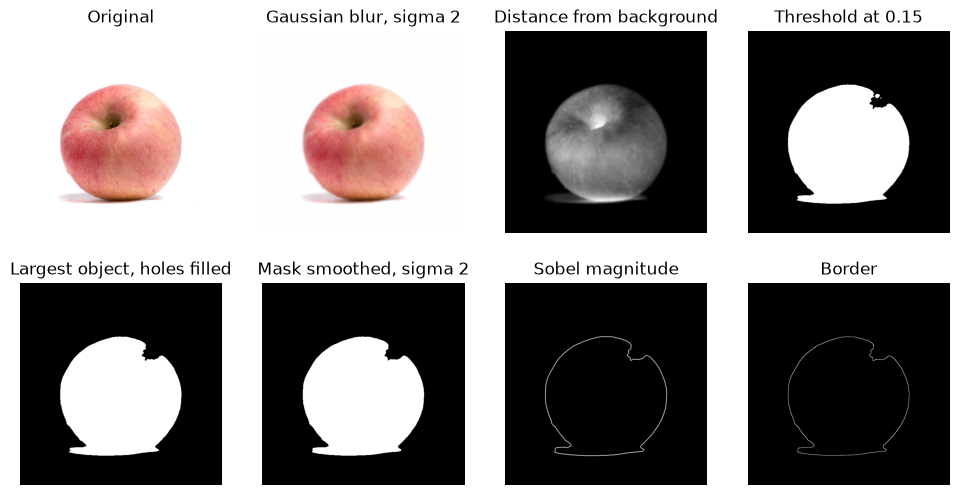
\includegraphics[width=\columnwidth]{04_transforms}}
        \caption{Filter stages for image 04. The shadow under the apple passes the threshold and joins the outline, and a pale patch near the stem falls below it and leaves a notch.}
        \label{fig:transforms}
    \end{figure}

    \subsection{Trajectory}\label{subsec:trajectory}
    Starting from the first border pixel, we repeatedly step to the nearest unvisited pixel, then resample the path to $N=500$ points uniformly by arc length (Fig.~\ref{fig:trajectory}).

    \begin{figure}[t]
        \centerline{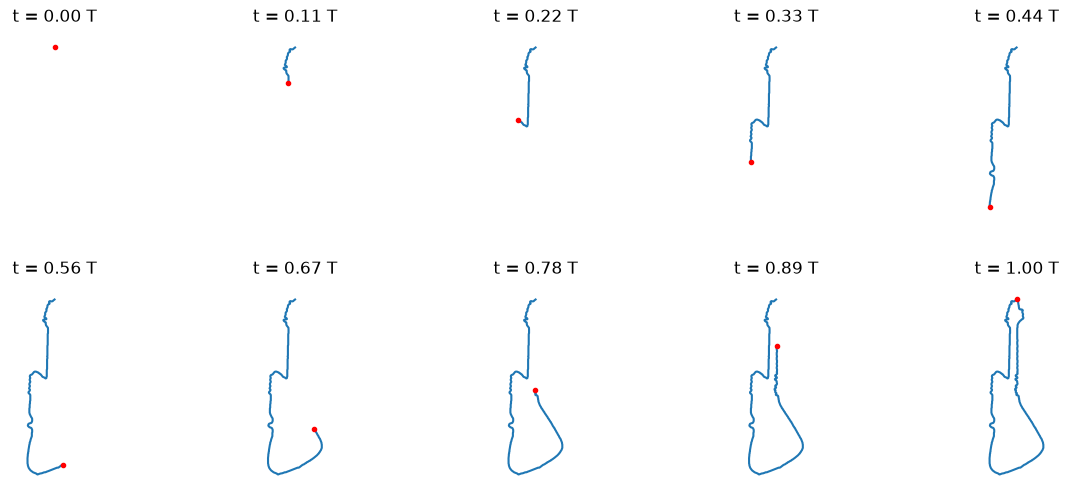
\includegraphics[width=\columnwidth]{03_trajectory}}
        \caption{Ordered path for image 03. The guitar's thin neck is the narrowest shape in our set and is still traced as one closed loop.}
        \label{fig:trajectory}
    \end{figure}

    \subsection{Fourier descriptors}\label{subsec:fourier-descriptors}
    The path becomes the complex signal $z[n]=x[n]+iy[n]$, with DFT(Discrete Fourier Transform) $Z[u]$ as per~\cite{foundationsCVbook}.
    We keep the set $S_K$ of the $K$ largest coefficients by $|Z[u]|$ and invert:
    \begin{equation}
        z'[n]=\frac{1}{N}\sum_{u\in S_K}Z[u]\,e^{2\pi i un/N}.\label{eq:equation}
    \end{equation}
    The DC term encodes the shape's position in the image.
    It was the largest coefficient on all five images (2.3--2.9 times the next), so it is always kept.

    Each remaining term becomes one epicycle.
    $|Z[u]|/N$ is its radius, $u$ its signed rotation speed and $\arg Z[u]$ its starting angle.
    Each video shows these epicycles drawing the outline at 20\% of the harmonics.
    Circles under 1 px in radius are computed but not drawn, since they wouldn't be visible at video resolution.

    \section{Design justifications}\label{sec:design-justifications}
    \begin{itemize}
        \item An object can share a background's brightness while differing in hue, and greyscale would discard that difference.
        \item We initially set $\sigma=6$ of the blur to suppress texture in photographs.
        On plain backgrounds this mostly rounds corners, so we reduced it.
        Table~\ref{tab:results} compares overlap (IoU) against a reference mask, made from the unblurred image at threshold 0.1 with the largest blob filled.
        The maple leaf's points gain the most, from 0.883 to 0.964.
        \item The fixed threshold was set to 0.15.
        An earlier automatic threshold chose the value where object area changed least, limited to objects covering 2-45\% of the image.
        On one earlier test image the object covered 52\%, so no candidate qualified, and it silently used a default.
        We replaced it with a fixed value.
        At 0.30, pale regions fell inside the background and the banana, guitar and apple scored 0.681, 0.769 and 0.773.
        At 0.15 they score 0.961, 0.951 and 0.965, while the leaf falls slightly from 0.981 to 0.964.
        The reference mask uses a threshold of 0.1, which favours lower values, so we also checked the outlines by eye.
        The value was chosen on the same images it is reported on, so it has no held-out validation.
        \item The largest blob is kept, not the one in the centre of the image.
        Our earlier code kept the blob nearest the image centre, which fails when the centre of the object matches the background.
        Choosing by size is shorter and avoids this.
        \item We use Sobel on the binary mask because any non-zero response marks a boundary, so no further gradient threshold is needed.
    \end{itemize}

    \section{Results}\label{sec:results}

    Table~\ref{tab:results} gives the Root Mean Square distance in pixels between $z$ and $z'$.
    Using all harmonics gives zero error.
    Fig.~\ref{fig:final} shows the leaf's detail returning as $K$ grows.
    At 5\% its lobes are rounded and its teeth are missing, and by 20\% the teeth are visible.
    Error follows outline complexity, with 11.54 px for the leaf at 5\% against 1.22 px for the smooth banana.

    \begin{table}[t]
        \caption{Mask overlap by blur level, and reconstruction error in pixels at the final settings}
        \begin{center}
            \begin{tabular}{|l|c|c|c|c|}
                \hline
                \textbf{Image} & \textbf{IoU, $\sigma$=6} & \textbf{IoU, $\sigma$=2} & \textbf{RMS, 5\%} & \textbf{RMS, 20\%} \\
                \hline
                00 banana      & 0.954                    & 0.961                    & 1.22              & 0.34               \\
                01 leaf        & 0.883                    & 0.964                    & 11.54             & 1.83               \\
                02 shoes       & 0.962                    & 0.989                    & 2.37              & 0.38               \\
                03 guitar      & 0.927                    & 0.951                    & 2.51              & 0.74               \\
                04 apple       & 0.953                    & 0.965                    & 2.48              & 0.45               \\
                \hline
            \end{tabular}
            \label{tab:results}
        \end{center}\label{tab:table}
    \end{table}

    \begin{figure}[t]
        \centerline{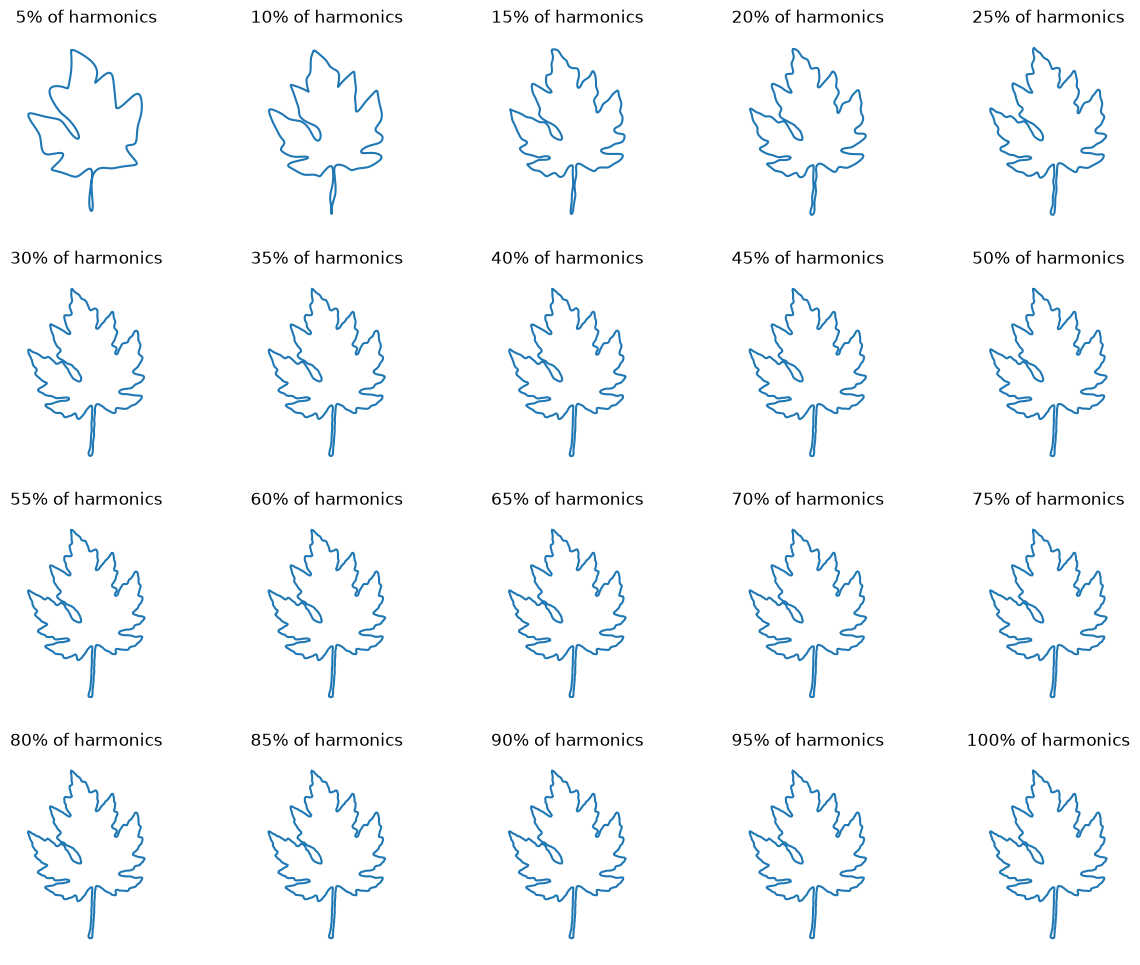
\includegraphics[width=\columnwidth]{01_final}}
        \caption{Image 01 rebuilt from 5\% to 100\% of its harmonics.}
        \label{fig:final}
    \end{figure}

    \section{Discussion and failure analysis}\label{sec:discussion-and-failure-analysis}

    Nearest-neighbour ordering drew a straight line across the leaf, guitar and apple.
    It skips a few border pixels at corners, because the border is not a strict one-pixel curve: 74-81\% of its pixels have more than two 8-neighbours.
    The walk then returns to them with a jump of up to 372 px at the end of the path.
    Because the DFT treats the signal as periodic, this behaves like a discontinuity and spreads a signal across all frequencies.
    Since we keep one filled blob and there is only one contour, we stop the walk at the first step above $\sqrt{8}$ px.
    This discards 1-4 pixels per image, and RMS at 5\% falls from 19.10 to 2.51 px on the guitar and from 23.38 to 2.48 px on the apple.
    Each path now closes within one resampling step.
    An object with separate parts would lose all but the first.

    A single threshold cannot separate a soft shadow from an object, and the apple's outline includes its shadow and loses a pale patch near the stem (Fig.~\ref{fig:transforms}).
    Raising the threshold removes the shadow but cuts into the pale skin.

    The method needs one object on a plain background.
    In cluttered scenes, a robin merged with its perch and a rugby ball lost a large section whose colour was close to the estimated background.
    At 0.15, two touching pears merged into one blob and a teapot on a black background failed to form a closed path, so we did not use them.
    These five images were selected partly because they work, so the results do not show that the method generalises to arbitrary photographs.

    Filling holes removes everything inside the silhouette, such as the laces on the shoes and the guitar's pickups.

    \subsection{Future work}\label{subsec:future-work}

    We would replace nearest-neighbour ordering with contour following to remove the stopping rule, handle several contours as separate Fourier series, and model the background per pixel.
    IoU should also be measured against hand-labelled masks, since our reference comes from the same image and shares its threshold bias.

    \section*{Image sources}
    All from Wikimedia Commons:
        Banana (white background), Justus Bl\"umer, CC BY 2.0;
        Autumn Silver Maple Leaf, Ninjatacoshell, CC BY-SA 3.0;
        2023 Adidas Yeezy 500 (1), Jacek Halicki, CC BY-SA 4.0;
        Burner Guitar, Yuri Landman, CC BY-SA 3.0;
        Apple picture, Mgmoscatello, CC BY-SA 3.0.
    All were scaled and padded.
    \printbibliography

\end{document}
